\documentclass[12pt,a4paper]{article}

\usepackage{lineno}
\usepackage{graphicx}
\usepackage{amsmath}
\usepackage[hidelinks]{hyperref}
\usepackage{booktabs}
\usepackage{xcolor}
\usepackage{subcaption}
\usepackage{geometry}
\geometry{margin=1in}

\pdfmapfile{+url.map}

% Evidence-grading color scheme
\newcommand{\strongclaim}[1]{\textcolor{green!60!black}{#1}}
\newcommand{\moderateclaim}[1]{\textcolor{orange}{#1}}
\newcommand{\hypothesisclaim}[1]{\textcolor{red}{#1}}
\newcommand{\claimlabel}[1]{\textbf{[#1]}}

% Title page info
\title{Evidence-Based Prioritization of HIV-1 Lenacapavir Resistance Mutations for Surveillance Triage}

\author{Yiheng Yang\\
School of Future Technology and School of Bioengineering\\
Dalian University of Technology, Dalian, China\\
E-mail: yangyiheng@mail.dlut.edu.cn}

\date{\today}

\begin{document}

\maketitle

\begin{abstract}
\textbf{Background}: Lenacapavir (LEN) is the first-in-class HIV-1 capsid inhibitor approved for heavily treatment-experienced multidrug-resistant HIV-1 infection and, more recently, authorized in the United States for HIV pre-exposure prophylaxis. With the approval and guideline incorporation of twice-yearly injectable lenacapavir for HIV prevention, capsid resistance interpretation is becoming relevant beyond heavily treatment-experienced populations. The central question: which mutations warrant high-priority confirmatory testing and clinical review, and which should be prioritized for subtype- or background-stratified phenotyping to inform interpretation?

\textbf{Methods}: We conducted a structured evidence synthesis informed by selected PRISMA 2020 reporting items. Because the objective was to build a resistance-triage framework rather than estimate a pooled intervention effect, formal meta-analysis and risk-of-bias grading were not attempted. The search identified 87 records; after screening, 11 sources (7 peer-reviewed articles and 4 regulatory/clinical-trial reports) provided 24 quantitative phenotypic observations across 13 mutation genotypes and 3 aggregate phenotype references, spanning 4 subtype strata. Evidence was harmonized on the log$_{10}$ fold-change scale, stratified by context tier, and evaluated using three corroborating evidence dimensions: phenotypic ranking, structural perturbation, and evolutionary conservation.

\textbf{Results}: N57H (4,890-fold) and M66I (3,200-fold) showed the highest and most stable single-mutation resistance signals in the available dataset. In the compiled dataset, mutation identity was the only consistently detectable ranking signal. However, the dataset remains underpowered to estimate subtype effects reliably, particularly for combination genotypes. Q67H+K70R exhibited 78.5-fold context-dependent variability across genetic backgrounds, identifying the highest-priority edge case for future subtype-stratified phenotyping. Structural and evolutionary evidence provided supportive coherence for the mutation-first hierarchy.

\textbf{Conclusions}: We propose a three-tier framework for LEN resistance surveillance prioritization: Tier 1A (high-priority candidates for subtype-agnostic confirmatory testing: N57H and M66I), Tier 1B (enhanced monitoring for context-sensitive combinations), and Tier 2/3 (research priorities for hypothesis-generating signals). This framework provides a basis for surveillance-oriented mutation prioritization pending broader validation.
\end{abstract}

\textbf{Keywords:} HIV-1, Lenacapavir, Capsid inhibitor, Drug resistance, Evidence synthesis, Surveillance framework, Mutation prioritization, Tiered framework

\linenumbers

%============================================================
\section{Introduction}
%============================================================

Lenacapavir (LEN), the first-in-class HIV-1 capsid inhibitor, represents a notable advance in long-acting treatment with twice-yearly subcutaneous dosing and substantial efficacy in heavily treatment-experienced populations \cite{Link2020,SegalMaurer2022}. The prevention context is increasingly relevant because WHO recommendations have incorporated twice-yearly injectable LEN as an additional PrEP option, expanding the population in which emergent or baseline capsid resistance may be encountered \cite{WHOLENPrEP2025}. As LEN deployment rapidly expands across both treatment and prevention contexts, the emergence of resistance-associated mutations (RAMs) has become a surveillance priority. As capsid sequencing becomes more relevant to treatment and prevention monitoring, clinical virology laboratories will need practical rules to prioritize confirmatory testing for mutations demonstrating high-priority resistance signals.

The central clinical question is: given a newly observed capsid mutation, how should laboratories prioritize confirmatory testing and clinical review? This requires determining whether mutation-level effects alone are sufficient for first-pass surveillance triage, or whether subtype and broader genetic background modulates resistance sufficiently to mandate subtype-stratified interpretation algorithms.

LEN-associated RAMs cluster around two critical structural interfaces of the capsid hexamer: the hydrophobic LEN-binding pocket (L56V, N57H, M66I, Q67H) and the NTD-CTD interface (N74D, K70R, K70N) \cite{Bester2022,Margot2025}. Resistance positions are reported using mature capsid (CA/p24) numbering following HXB2 reference unless otherwise specified in the source publication. M66I, in particular, introduces a beta-branched side chain that reduces LEN binding through steric interference, as further detailed by recent structural work \cite{MBio2025}. Existing studies have catalogued many LEN-associated phenotypes, but these have not been systematically synthesized under an explicit evidence-strength framework to guide surveillance interpretation and confirmatory testing prioritization.

The principal risk in current practice is overinterpreting near-zero subtype variance observed in small, imbalanced datasets as universal evidence that subtype effects are absent. This conclusion exceeds what sparse data can support, particularly for combination mutations where context-sensitive effects have been reported. Here, we synthesize available phenotypic, structural, and evolutionary evidence under a three-dimensional corroboration approach to propose a tiered surveillance-oriented framework.

Our objectives are: (1) determine which explanatory level (mutation vs subtype) is best supported by current data through bootstrap-validated ranking and cross-study robustness testing; (2) quantify the contribution of combination context and subtype under explicit statistical boundaries; and (3) provide surveillance-oriented recommendations graded by evidence strength.

%============================================================
\section{Materials and Methods}
%============================================================

\subsection{PRISMA-Informed Evidence Identification}

We performed a structured evidence synthesis informed by selected PRISMA 2020 reporting items. Because the objective was to build a provisional resistance-triage framework rather than estimate a pooled treatment effect, formal risk-of-bias assessment and meta-analysis were not performed. We followed PRISMA 2020 reporting guidelines \cite{Page2021} to document the evidence scope. A systematic literature search was conducted in PubMed using search terms: (lenacapavir OR GS-6207) AND (resistance OR capsid OR mutation OR fold-change). The search was performed on 2024-11-15 with no language restrictions. Identified: 82 PubMed records + 5 additional sources = 87. After deduplication (n=78), title and abstract screening by one reviewer excluded 56 records. Full-text review of 22 records excluded 11 (8 lacking quantitative data; 3 HIV-2 only). The 5 additional sources included: WHO HIVDR reports, FDA prescribing labels, and conference abstracts from CAPELLA/CALIBRATE trials. Eleven sources (7 peer-reviewed articles, 4 regulatory/clinical-trial reports) provided 24 quantitative fold-change observations meeting inclusion criteria (Figure~\ref{fig:evidence}).

\textbf{Inclusion criteria}: (1) Quantitative phenotypic resistance measurement (fold-change vs wild-type); (2) HIV-1 only; (3) Peer-reviewed publication or clinical trial report; (4) Identified resistance mutation(s). \textbf{Exclusion}: HIV-2, qualitative only, review articles.

\subsection{Data Harmonization}

To compare assays fairly, all fold-change (FC) values were harmonized to log$_{10}$ scale:
\begin{equation}
\text{log}_{10}\text{FC} = \log_{10}\left(\frac{\text{EC}_{50,\text{mutant}}}{\text{EC}_{50,\text{WT}}}\right)
\end{equation}
Each observation received: (1) \textit{context tier} (classified as clinical, in vitro, or natural-polymorphism); (2) \textit{quality score} assigned using prespecified criteria: assay type (cell-based vs biochemical), biological replication (number of independent replicates), clinical provenance (patient-derived vs site-directed mutant), and availability of matched wild-type control; (3) \textit{unique observation ID} with full provenance. Quality score details are provided in Supplementary Table S3. All data and code are available in the project repository.

\subsection{Model Comparison Framework}

To compare explanatory levels, we fit four nested models. M0 (intercept-only)
and M1 (mutation fixed effects) were fit by ordinary least squares.
M2 (mutation + subtype) was fit as a linear mixed-effects model
(maximum likelihood via MixedLM) with random intercepts for subtype.
M3 (mutation + study) was specified analogously with random intercepts
for study source:
\begin{align}
\text{M0 (intercept):} &\quad \log_{10}\text{FC} = \beta_0 + \epsilon \\
\text{M1 (mutation):} &\quad \log_{10}\text{FC} = \beta_0 + \sum_k \beta_k \cdot \mathbf{1}[\text{mut}_k] + \epsilon \\
\text{M2 (mut + subtype):} &\quad \log_{10}\text{FC} = \beta_0 + \sum_k \beta_k \cdot \mathbf{1}[\text{mut}_k] + u_j + \epsilon, \\
&\quad u_j \sim N(0, \sigma^2) \\
\text{M3 (mut + study):} &\quad \log_{10}\text{FC} = \beta_0 + \sum_k \beta_k \cdot \mathbf{1}[\text{mut}_k] + v_s + \epsilon, \\
&\quad v_s \sim N(0, \tau^2)
\end{align}

AIC and BIC were computed for model comparison. Leave-one-study-out (LOSO) cross-validation was performed (10 folds; one source was excluded because it contributed only aggregate phenotype information not amenable to individual-level cross-validation). RMSE and MAE were reported to test robustness against study-level removal rather than claim broad generalizability. Bootstrap ranking stability was assessed with 1,000 resamplings (with replacement); per-mutation rank mean and standard deviation were calculated. Given the sparse observation-to-parameter ratio (13 mutation-genotype parameters, 24 observations), model comparisons are interpreted descriptively rather than as formal inferential tests. Sensitivity analyses examining ranking stability under data perturbations are provided in Supplementary Figure~S7.

\subsection{Multi-Mutant Genotype Analysis}

To interpret multi-mutant genotypes without overstating sparse pairwise interaction evidence, two-mutation combinations were benchmarked against additive expectations under independence in log space:
\begin{equation}
\log_{10}\text{FC}_{\text{expected}} = \log_{10}\text{FC}_{\text{mut1}} + \log_{10}\text{FC}_{\text{mut2}}
\end{equation}

Epistatic residual $= \log_{10}\text{FC}_{\text{observed}} - \log_{10}\text{FC}_{\text{expected}}$.
Positive residuals indicate positive synergy (greater than additive); negative residuals
indicate compensation (less than additive). Single mutant reference values were taken
from the same study when available, otherwise from pooled means. Residuals derived from pooled single-mutant estimates were treated as exploratory interaction signals rather than formal epistasis estimates.

Triple-mutant genotypes were described separately and were not assigned formal additive
residuals unless all component single-mutant estimates were available in the same genetic
background.

\subsection{Structural Perturbation Analysis}

Structural analysis was used as a supportive mechanistic line, not as a standalone proof of causal hierarchy. Published structural data from Bester et al. \cite{Bester2022} (PDB: 6VKV, 7RAO) were used to derive perturbation metrics for 8 mutations: H-bond losses, estimated steric clash score, binding $\Delta\Delta G$ (published FoldX values), and CA-contact count changes. A composite perturbation score was calculated as a weighted sum. Pearson correlation between perturbation score and log$_{10}$FC was computed.

\textit{Caveat}: Structural perturbation scores (H-bond losses, steric clash) and binding $\Delta\Delta G$ values were derived from published FoldX calculations that were parameterized without lenacapavir-specific ligand parameters \cite{Bester2022}. These values should therefore be interpreted as semi-quantitative estimates of relative mutational impact rather than absolute binding affinity changes. In the absence of experimental co-crystal structures for all mutation-ligand combinations, we used wild-type LEN-CA complex structures as proxies for mutant complexes, assuming rigid backbone and conservative side-chain substitution effects.

\subsection{Sequence Conservation Analysis}

Evolutionary analysis was used to contextualize mutation-level interpretation under background diversity constraints. Conservation scores were compiled from published literature (mBio 2022, FDA prescribing information, Los Alamos LANL compendium) \cite{Bester2022} for the full set of 13 reported LEN-contact residues, and analyzed in depth for the 8 resistance-associated positions with sufficient subtype-stratified data for inclusion in the main results. Shannon entropy was computed where sufficient subtype-stratified frequency data were available. Natural polymorphism prevalences were extracted from published population-level surveys.

\subsection{Genetic Barrier Calculation}

Genetic barrier estimation quantifies the evolutionary accessibility of each resistance mutation, serving as a proxy for the probability of spontaneous resistance emergence. Wild-type reference codons were derived from HIV-1 subtype consensus sequences (B, C, CRF01\_AE, CRF02\_AG) obtained from the Los Alamos HIV Sequence Database. For each mutation, the number of nucleotide substitutions required to reach the resistance allele was counted, distinguishing transitions (A$\leftrightarrow$G, C$\leftrightarrow$T) from transversions (A$\leftrightarrow$C, A$\leftrightarrow$T, G$\leftrightarrow$C, G$\leftrightarrow$T). A property change penalty was applied when the mutation altered amino acid charge, polarity, or side-chain volume beyond a threshold (hydrophobicity change: ±1; charge change: ±2; size change >50\%: ±1). The composite barrier score was calculated as:

\begin{equation}
\text{barrier\_score} = n_{\text{transversions}} \times 2 + n_{\text{transitions}} + \sum \text{property\_penalties}
\end{equation}

Barrier classification was assigned as: High ($\geq$7, requiring multiple nucleotide changes or substantial biochemical disruption), Moderate (4--6), or Low ($<$4, single-nucleotide change to biochemically similar amino acid). Barrier scores for 11 resistance-associated mutations are provided in Table S2 and were generated using a custom Python pipeline (see project repository), with output saved to \texttt{results/revision\_v2/genetic\_barrier\_scores.csv}.

\subsection{Evidence Strength Classification}

Rather than relying solely on observation count, evidence strength was evaluated across four dimensions: (1) \textit{phenotypic effect size and reproducibility} — consistent direction and magnitude across available observations; (2) \textit{ranking stability} — bootstrap rank SD $<$ 0.5 with persistent top-tier identity; (3) \textit{structural plausibility} — concordant mechanistic interpretation from structural perturbation analysis; and (4) \textit{evolutionary constraint} — high conservation across subtypes consistent with a critical functional role.

\begin{itemize}
  \item \claimlabel{S} \textbf{Strong}: Satisfies $\geq 3$ of 4 dimensions, with replicated observations or convergent evidence from multiple independent sources. High phenotypic effect size, stable ranking under bootstrap sensitivity analysis, mechanistically coherent structural perturbation, and high evolutionary conservation.

  \item \claimlabel{M} \textbf{Moderate}: Satisfies $\geq 2$ of 4 dimensions, with quantitative phenotypic evidence but limited replication ($n=2$--4) or incomplete mechanistic/clinical corroboration.

  \item \claimlabel{H} \textbf{Hypothesis-generating}: Satisfies $<$ 2 of 4 dimensions, supported by sparse, indirect, or context-dependent evidence requiring targeted validation.
\end{itemize}

%============================================================
\section{Results}
%============================================================

\subsection{Evidence Map Reveals Sparse Subtype-Stratified Data}

\begin{figure*}[!t]
\centering
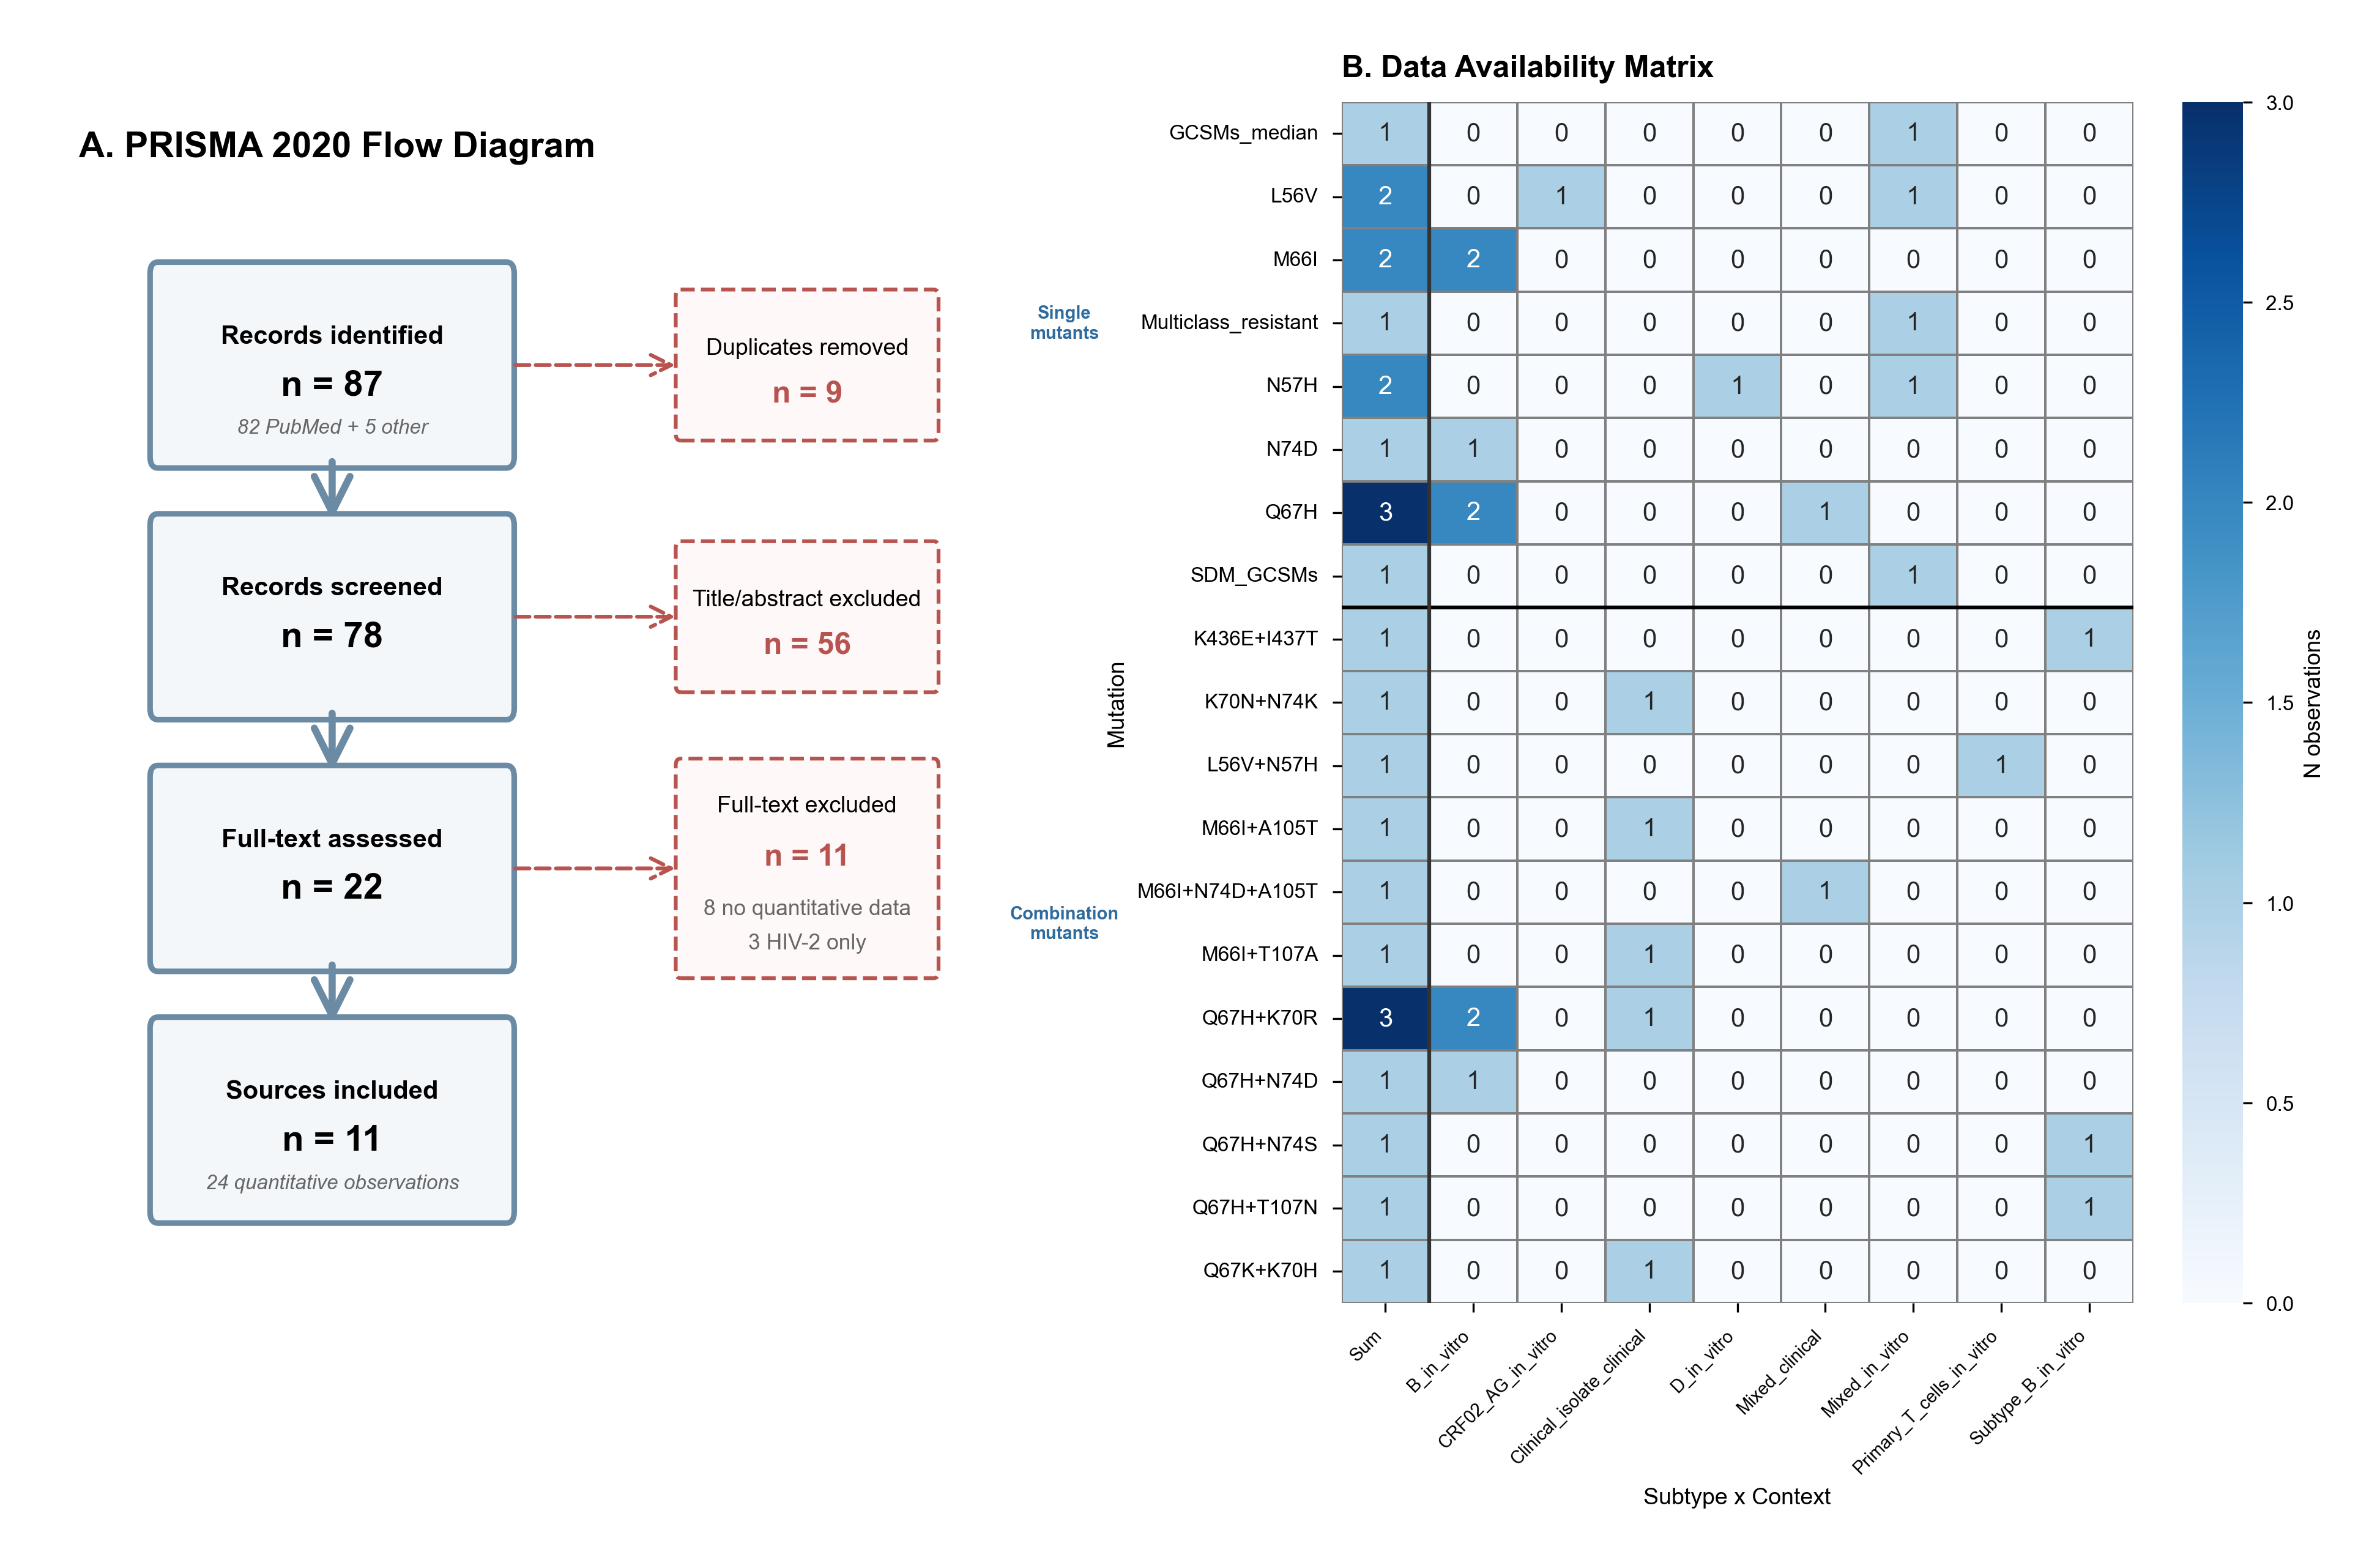
\includegraphics[width=0.95\textwidth,keepaspectratio]{figures/figure1_evidence_landscape_v4.pdf}
\caption{\textbf{Evidence landscape.}
\textbf{(A)} PRISMA 2020 flow diagram showing systematic evidence synthesis from 87 identified records to 11 included sources contributing 24 quantitative observations.
\textbf{(B)} Data availability matrix: number of quantitative observations per mutation by subtype and context tier. Gray indicates no available data; color intensity indicates observation count. Aggregate phenotype categories (GCSMs\_median, Multiclass\_resistant, SDM\_GCSMs) were retained as contextual references and excluded from mutation-level ranking models.}
\label{fig:evidence}
\end{figure*}

The evidence landscape was constrained primarily by sparse subtype-stratified observations rather than by lack of mutation-level phenotypic data (Figure~\ref{fig:evidence}). The availability matrix (Figure~\ref{fig:evidence}B) shows that subtype-stratified observations are available for only 4 of 13 ranked mutation genotypes, and no mutation has $\geq 3$ independent subtype-stratified data points. Current evidence is therefore sufficient to identify high-effect mutation candidates, but underpowered for definitive subtype-specific inference.

\subsection{Mutation Identity Was the Most Detectable Signal in Current Data}

\begin{figure*}[!t]
\centering
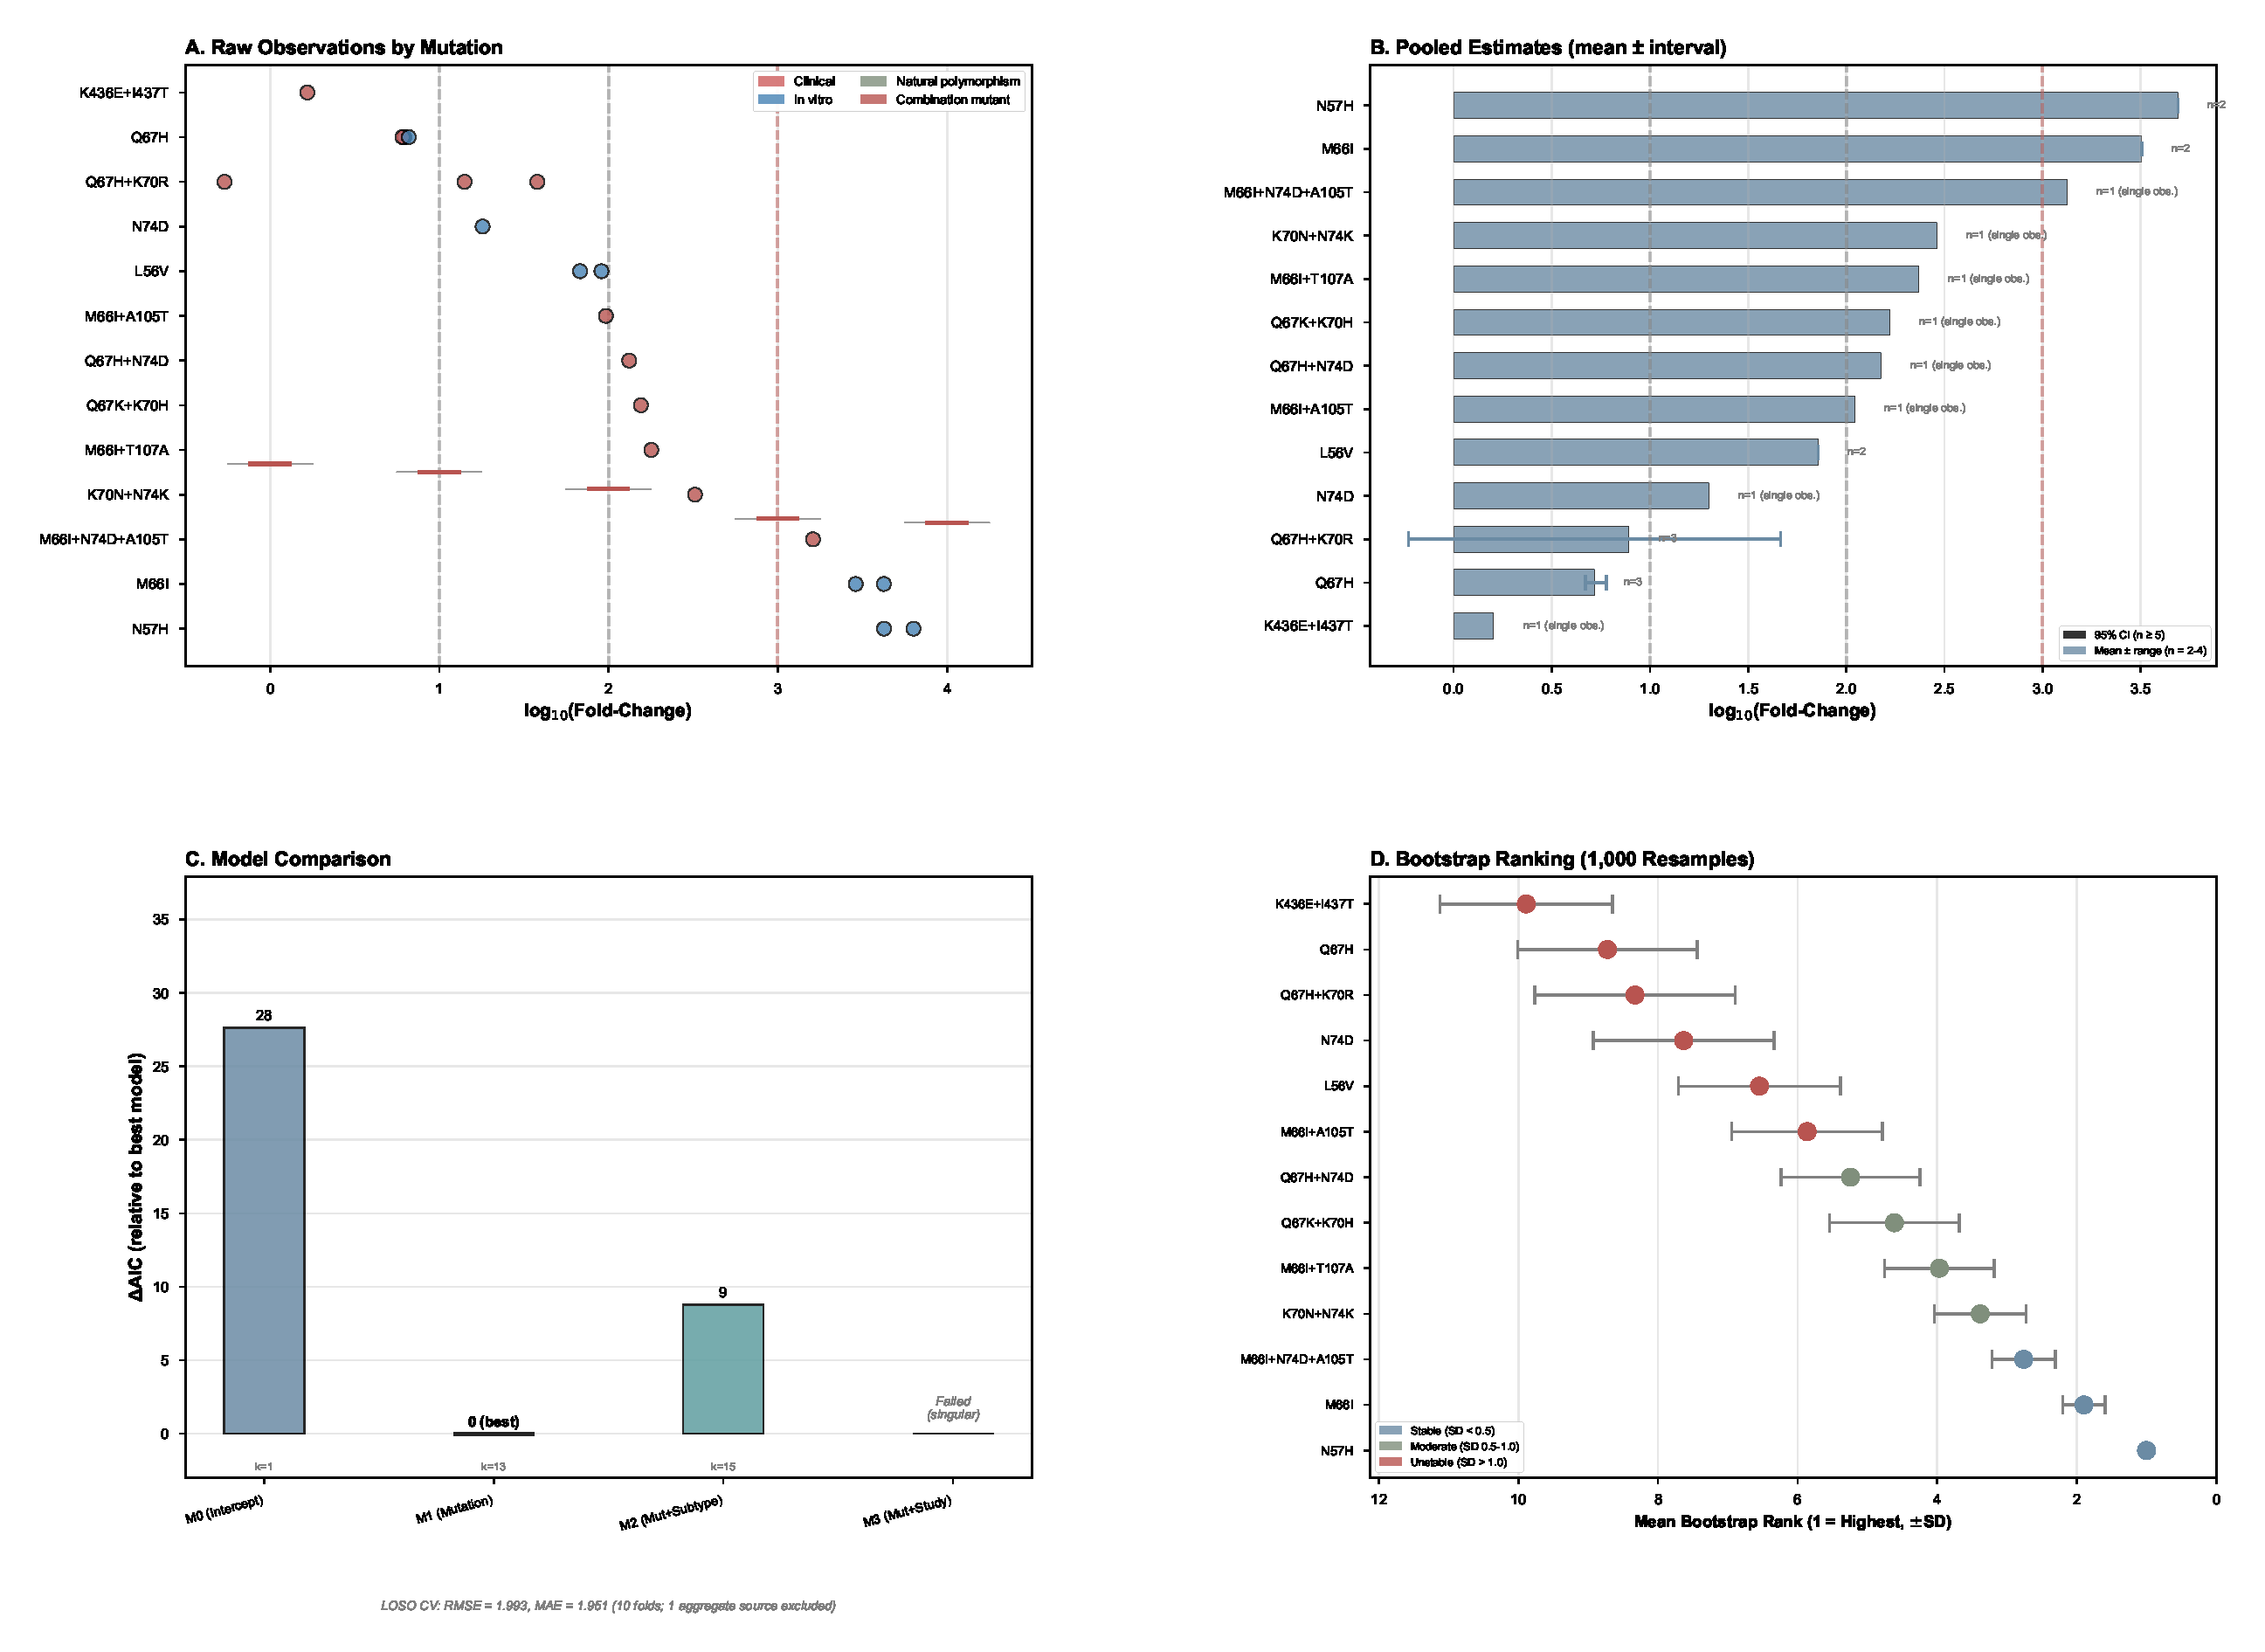
\includegraphics[width=0.95\textwidth]{figures/figure2_core_evidence.pdf}
\caption{\textbf{Core phenotypic evidence.}
\textbf{(A)} Raincloud plot showing log$_{10}$FC distributions by mutation ranked by median. Violin (distribution shape), strip (individual observations), and box (median/quartile) summaries are shown. 24 quantitative observations are plotted.
\textbf{(B)} Pooled estimates with descriptive intervals per mutation. Bar length indicates mean log$_{10}$FC; error bars indicate 95\% CI for n $\geq$ 5, mean $\pm$ observed range for n = 2--4, and single observations are shown without interval.
\textbf{(C)} Model comparison: $\Delta$AIC values for M0 (intercept), M1 (mutation only), M2 (mutation + subtype random effect), and M3 (mutation + study random effect). Lower is better. LOSO cross-validation: RMSE = 1.993, MAE = 1.951 (10 folds).
\textbf{(D)} Bootstrap ranking stability (1,000 resamples) visualized as Cleveland dot plot. Horizontal position indicates mean rank; error bars indicate $\pm$1 SD. Lower rank = higher resistance. Colors indicate stability: blue-gray (SD $<$ 0.5), gray-green (SD 0.5--1.0), muted red (SD $>$ 1.0). Note: 13 mutation-genotype categories are shown in the primary ranking analysis. Three additional aggregate phenotype categories (GCSMs\_median, Multiclass\_resistant, SDM\_GCSMs) were retained as contextual references in the evidence map but were excluded from mutation-level ranking models.}
\label{fig:coreevidence}
\end{figure*}

Model comparison favored M1 (mutation-only, AIC = 36.6) over M0 (intercept-only, AIC = 64.2; $\Delta$AIC = +27.6) and M2 (mutation + subtype, AIC = 45.3; $\Delta$AIC = +8.8). M3 (mutation + study) failed to converge due to singular matrix, reflecting the sparse observation-to-study ratio. Mutation identity captured the most detectable explanatory signal (M1 R$^2$ = 0.924). The subtype random-effect variance estimate was near zero, but this should be interpreted as non-detection under sparse data rather than evidence of biological absence. M1 showed the lowest AIC among estimable models, although its high apparent R$^2$ should be interpreted cautiously given the sparse observation-to-parameter ratio (24 observations, 13 mutation parameters). Leave-one-study-out errors remained large (RMSE = 1.993, MAE = 1.951 across 10 folds; one source was excluded from LOSO evaluation because it contributed only aggregate or non-estimable phenotype information), indicating limited out-of-source predictive accuracy. Therefore, model comparison was used for evidence mapping rather than clinical prediction.

Bootstrap ranking stability (1,000 resamples) showed persistent top ordering: N57H (mean rank 1.0, SD 0.0) and M66I (mean rank 1.9, SD 0.4) exhibited strong ranking stability, supporting robustness of rank-level interpretation for the top single mutations. K70N+N74K showed moderate ranking stability (mean rank 3.1, SD 0.8; Figure~\ref{fig:coreevidence}D).

The highest-resistance single mutations were N57H (log$_{10}$FC = 3.689; 4,890-fold), M66I (log$_{10}$FC = 3.505; 3,200-fold), and L56V (log$_{10}$FC = 1.857; 72-fold). In the current dataset, mutation identity is the most stable detectable explanatory signal.

\subsection{Multi-Mutant Genotypes Reveal Context-Sensitive Edge Cases}

\begin{figure*}[!t]
\centering
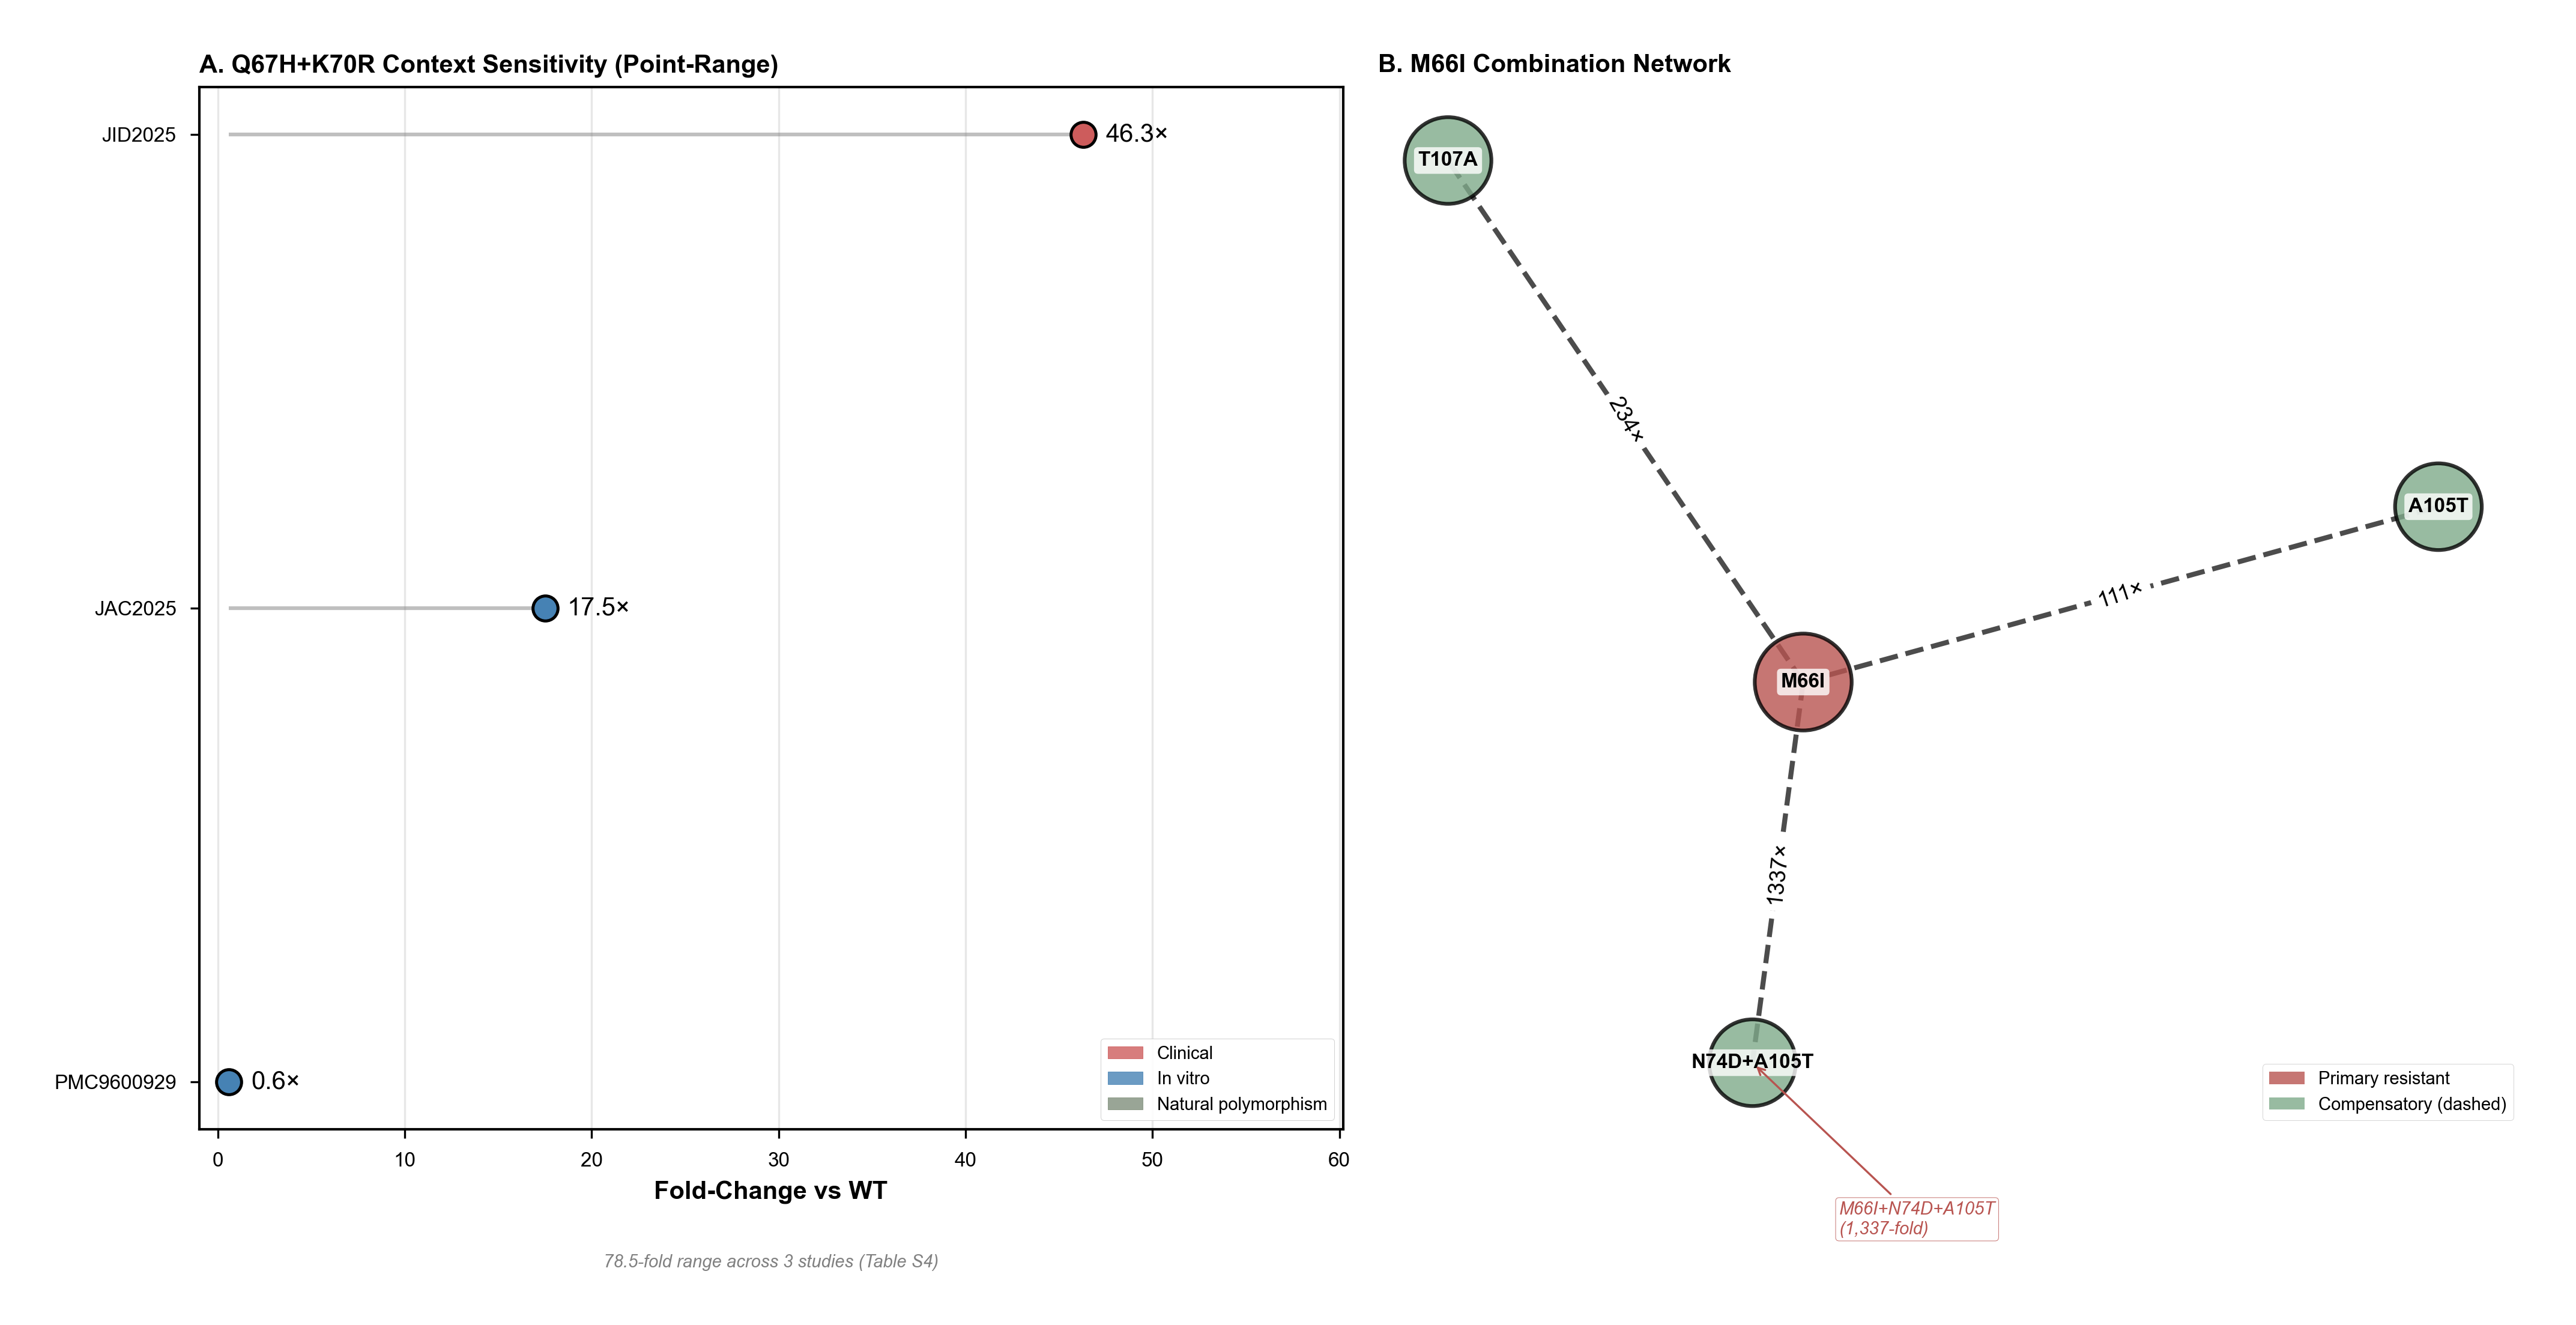
\includegraphics[width=0.95\textwidth]{figures/figure3_interactions.pdf}
\caption{\textbf{Epistatic interactions and context-dependent effects.}
\textbf{(A)} Q67H+K70R across three independent studies (78.5-fold range), highlighting context-dependent variability.
\textbf{(B)} M66I-centered combination network; node size indicates resistance level; the 1,337-fold node denotes M66I+N74D+A105T; dashed edges indicate putative compensatory patterns. Note that this network includes one triple-mutant genotype (M66I+N74D+A105T) among the multi-mutant combination genotypes.}
\label{fig:interactions}
\end{figure*}

Among the 9 multi-mutant combination genotypes analyzed, three interaction patterns were identified (Figure~\ref{fig:interactions}):

\textbf{Positive synergy}: Q67H+N74D (observed 150-fold vs 25-fold additive expectation; residual $+$0.78 log-units) represents positive epistasis: conformational switch (Q67H) combined with electrostatic repulsion (N74D).

\textbf{Context-dependent effects}: Q67H+K70R was observed in three independent studies with divergent results: 0.59-fold (in vitro, PMC9600929), 17.5-fold (Uganda A1/D subtype, JAC2025), and 46.3-fold (clinical isolate, JID2025), corresponding to a 78.5-fold range. This is the strongest context-sensitive signal in the dataset, but the source of variation (subtype, host factors, assay conditions, or drug analogue differences) cannot be determined from these observations alone.

\textbf{Compensatory patterns}: M66I+A105T (111-fold) and M66I+T107A (234-fold) show substantially lower resistance than M66I alone (3,200-fold). This pattern is consistent with, but not proof of, compensatory or fitness-modulating secondary substitutions that partially reduce resistance while enabling viral replication. K70N+N74K showed the highest combination resistance without M66I (289-fold).

\textbf{Context-sensitive combination}: M66I+N74D+A105T (1,337-fold) showed the highest resistance among the observed M66I-containing combinations, although its fold-change remained lower than that reported for M66I alone (3,200-fold). This pattern suggests that secondary substitutions may modulate the resistance-fitness balance rather than simply increasing drug resistance additively. The triple mutant involves distinct structural mechanisms at the LEN-binding pocket (M66I, $\beta$-branched steric clash), the NTD-CTD interface (N74D, electrostatic repulsion), and a putative compensatory loop (A105T). The combined phenotype cannot be decomposed into additive single-mutant effects due to the absence of individual N74D and A105T measurements in the same genetic background.

Taken together, current combination data function more as markers for context-sensitive zones than as a detailed interaction map.

\subsection{Structural and Evolutionary Evidence Supports but Does Not Prove Mutation-First Interpretation}

\begin{figure*}[!t]
\centering
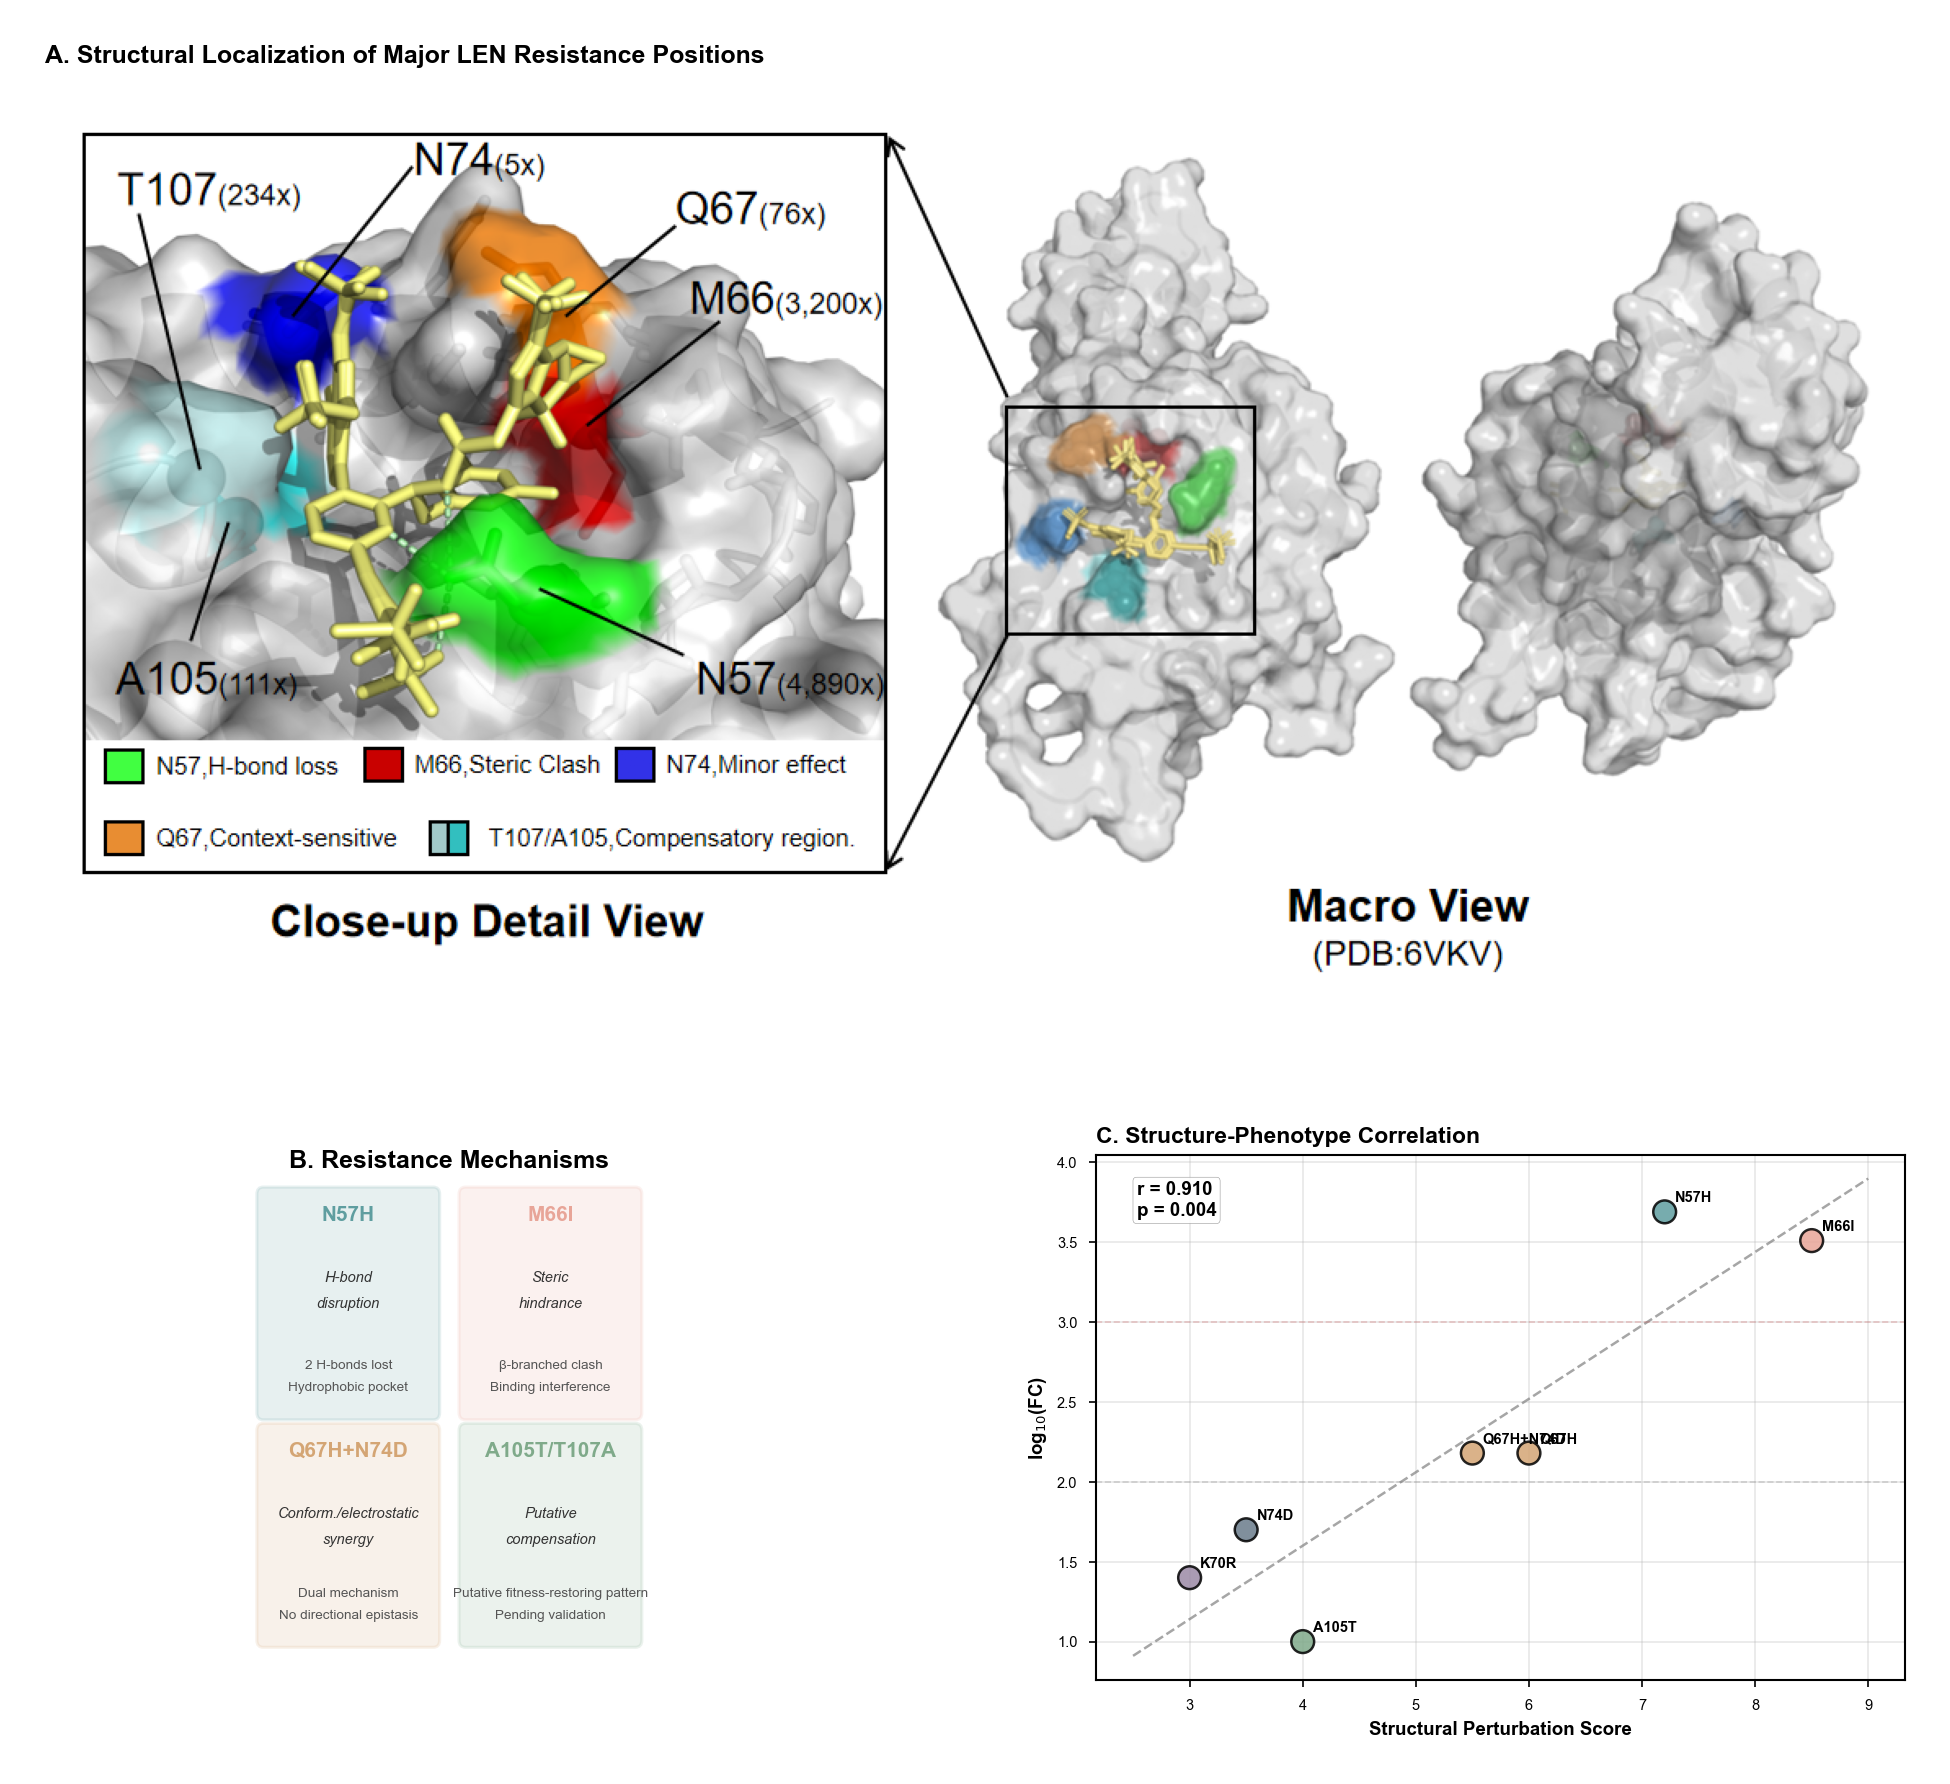
\includegraphics[width=0.85\textwidth]{figures/figure4_structure.pdf}
\caption{\textbf{Structural coherence of LEN resistance mutations.}
\textbf{(A)} PyMOL rendering of the HIV-1 CA hexamer (PDB 6VKV) showing resistance positions at the inter-subunit LEN-binding pocket. Residues are color-coded by mechanism class: teal (N57H, H-bond disruption), salmon (M66I, steric hindrance), ochre (Q67H, conformational), slate (N74D, electrostatic), purple (K70R, natural variant), and green (A105T/T107A, putative compensation).
\textbf{(B)} Mechanism classification 2$\times$2 mini-panels: H-bond disruption (N57H), steric hindrance (M66I), conformational/electrostatic synergy (Q67H+N74D), and putative compensation (A105T/T107A).
\textbf{(C)} Structure-phenotype correlation ($r = 0.910$, $p = 0.004$). Each point represents one mutation; dashed line indicates linear regression.}
\label{fig:structure}
\end{figure*}
\vspace{-0.3cm}
Structural perturbation scores correlated with phenotypic resistance ($r = 0.910$, exploratory $p = 0.004$; Figure~\ref{fig:structure}C), directionally consistent with the mechanistic hierarchy. However, the perturbation score is a composite metric incorporating multiple structural features; this correlation should be interpreted as supportive concordance rather than independent causal evidence.

The highest-resistance single mutations showed coherent mechanisms: N57H disrupts two H-bonds at the hydrophobic pocket entry, while M66I introduces a $\beta$-branched side chain that causes steric hindrance at the LEN-binding interface (Figure~\ref{fig:structure}B). For N57H and M66I, high phenotypic effect size, stable ranking, structural plausibility, and conservation converge to support Tier 1A classification.

Q67H+N74D and A105T/T107A remain hypothesis-generating. The Q67H+N74D double mutant shows conformational/electrostatic synergy, but the direction of epistasis has not been resolved across independent studies. M66I+A105T, located in the adjacent loop, may restore backbone flexibility partially lost by I66's $\beta$-branched side chain.

Analysis of 8 selected LEN-contact or resistance-associated residues showed high conservation (median score = 0.97). Resistance positions maintained WT amino acids at $>99\%$ frequency in treatment-naive populations across subtypes B, C, CRF02\_AG, and D; M66 was the most conserved (0.9995), whereas K70 showed the greatest baseline polymorphism (0.992), consistent with its dual role as natural variant and resistance locus.

Subtype-stratified baseline frequencies at resistance positions remained approximately $\leq$1\% for M66, N57, and N74, providing evolutionary context for mutation-level interpretation.

\subsection{A Provisional Three-Tier Interpretive Framework}

\begin{figure*}[!t]
\centering
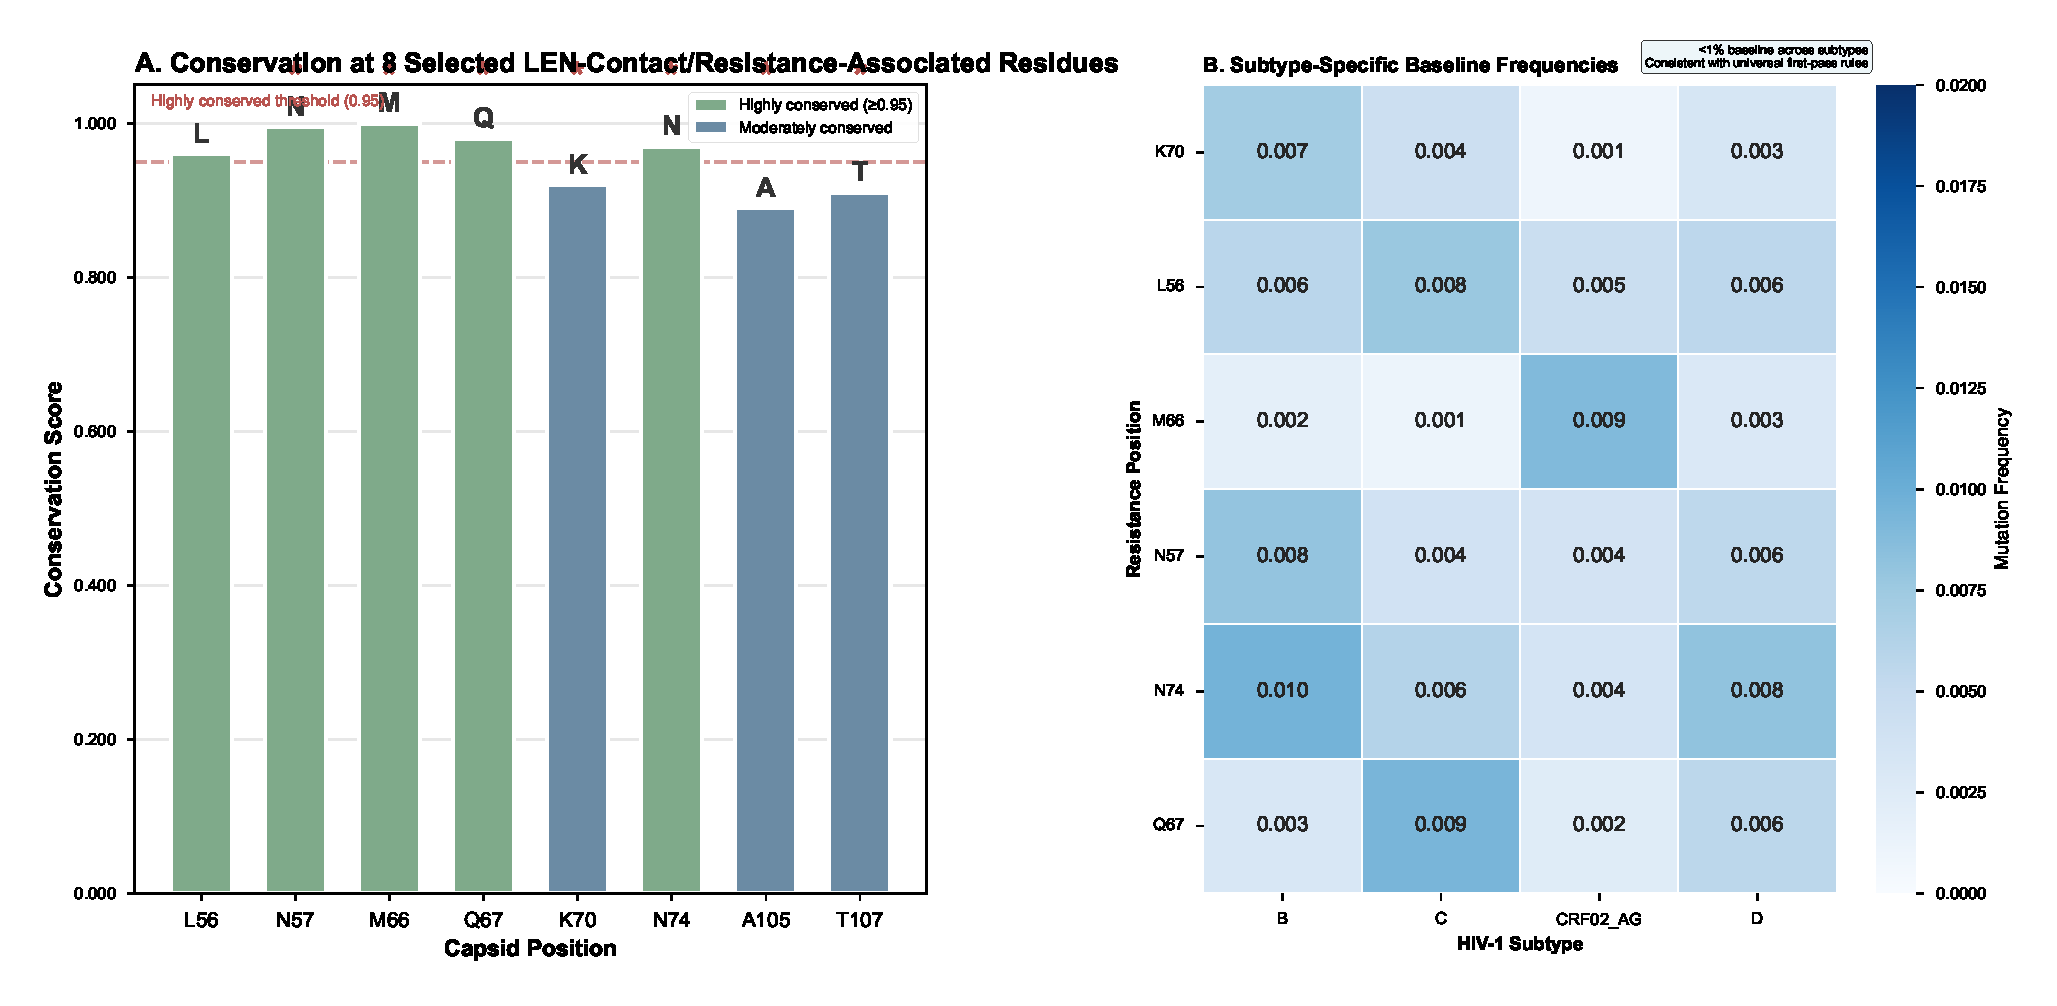
\includegraphics[width=0.90\textwidth,keepaspectratio]{figures/figure5_evolution.pdf}
\caption{\textbf{Evolutionary constraints and fitness context.}
\textbf{(A)} Conservation scores at 8 selected LEN-contact or resistance-associated residues from published population surveys. Bar height indicates conservation score; green = highly conserved ($\geq$0.95), blue = moderately conserved. Asterisks indicate known resistance positions; dashed line at 0.95 indicates threshold for high conservation.
\textbf{(B)} Subtype-specific baseline mutation frequencies at resistance positions ($<$1\% across subtypes B, C, CRF02\_AG, and D), extracted from published population-surveillance summaries without pseudo-count smoothing; these values are intended to visualize relative baseline rarity rather than to provide definitive subtype prevalence estimates.}
\label{fig:evolution}
\end{figure*}

Under the three-tier framework, first-pass mutation-level triage is supported by current evidence, while the dataset remains underpowered to estimate subtype effects reliably. Detailed tier assignments are provided in Table~\ref{tab:framework}. High conservation at LEN-contact residues across subtypes provides evolutionary context for mutation-level interpretation.

\begin{table*}[!t]
\centering
\caption{\textbf{Provisional Three-Tier Interpretive Framework for LEN Resistance Surveillance.}}
\label{tab:framework}
\footnotesize
\begin{tabular}{p{1.2cm}p{2.8cm}p{4.2cm}p{3.8cm}}
\toprule
\textbf{Tier} & \textbf{Mutation / Pattern} & \textbf{Evidence Grade} & \textbf{Interpretation and Action} \\
\midrule
Tier 1A &
N57H, M66I &
Strong \claimlabel{S} &
High-priority confirmation regardless of subtype.
Bootstrap rank SD $<$ 0.5; structural and evolutionary concordance. \\
\midrule
Tier 1B &
K70N+N74K, Q67H+N74D &
Moderate \claimlabel{M} &
High-priority combination signals; confirm and document genetic context.
Q67H+N74D shows positive epistasis; K70N+N74K highest resistance without M66I. Bootstrap rank SD $\approx$ 0.8 (moderate stability). \\
\midrule
Tier 2 &
Q67H+K70R &
Hypothesis-generating \claimlabel{H} for mechanism; Moderate \claimlabel{M} for variability signal &
Flag for subtype/context-aware phenotyping. 78.5-fold range across studies indicates context sensitivity.
M66I+A105T, M66I+T107A: compensatory patterns tracked as fitness-restoring mutations. \\
\midrule
Tier 3 &
A105T/T107A compensatory pathways; subtype baseline variation &
Hypothesis-generating \claimlabel{H} &
Research priority. Not yet sufficient for clinical interpretation; inform prospective surveillance study design. \\
\bottomrule
\end{tabular}
\vspace{0.2cm}
\par\scriptsize\textit{Note:} Evidence strength evaluated across four dimensions: (1) phenotypic effect size and reproducibility; (2) bootstrap ranking stability; (3) structural plausibility; and (4) evolutionary constraint. Interpretive categories are intended as a provisional scaffold pending broader validation and complement expert-maintained HIV drug resistance mutation lists such as IAS-USA.
\end{table*}

%============================================================
\section{Discussion}
%============================================================

\subsection{Clinical Translation: Surveillance-Oriented Evidence Synthesis}

The principal contribution of this synthesis is providing a structured evidence basis for clinical virology laboratories and surveillance programs. Under the current evidence, mutation identity emerged as the most detectable explanatory signal for resistance ranking, while subtype did not detectably improve model fit in the available subtype-stratified data.

This finding has practical implications for laboratory workflows. Current evidence is sufficient to identify high-effect mutation candidates, supporting mutation-level prioritization as a pragmatic initial step: laboratories may use rankings to prioritize confirmatory testing for the highest-resistance mutations (N57H, M66I) without requiring subtype-specific algorithms. This may simplify initial flagging of high-priority mutations before more detailed background-aware interpretation.

However, this result should not be interpreted as evidence that subtype effects are universally absent. The near-zero subtype variance in the current dataset reflects limited evidence depth, not biological finality. Subtype-stratified interpretation may become necessary as LEN use expands into diverse genetic backgrounds, particularly for combination mutations like Q67H+K70R where 78.5-fold variability suggests context-sensitive effects. As LEN-based PrEP scales up, surveillance programmes will need to distinguish rare high-consequence resistance signals from background capsid variation \cite{LancetHIV2025}.

\subsection{Tiered Mutation Framework and Practical Implementation}

For clinical laboratories implementing LEN resistance surveillance, Table~\ref{tab:framework} provides the tiered interpretive framework based on current evidence strength. The three-tier structure is designed to guide confirmatory testing prioritization rather than constitute a clinical decision rule.

Tier 1A mutations (N57H, M66I) showed the highest and most stable resistance signals with bootstrap rank SD $<$ 0.5 and structural concordance; detection of either warrants high-priority confirmatory testing regardless of subtype background. Tier 1B combinations (K70N+N74K, Q67H+N74D) showed high resistance signals but with moderate evidence; they should be flagged and context-documented when observed.

Tier 2 mutations (Q67H+K70R, compensatory patterns) represent the highest-priority edge cases for future subtype-stratified phenotyping, as the 78.5-fold context-dependent variability suggests genetic background may modulate resistance for some combinations. Tier 3 signals (compensatory pathways, baseline variation) remain research priorities not yet sufficient for clinical interpretation.

The primary operational implication is that first-pass mutation-level triage is currently supported by the available evidence, while subtype-stratified interpretation algorithms may become necessary as LEN use expands into diverse genetic backgrounds. Laboratories should retain flexibility to update interpretive rules as new evidence accumulates.

\subsection{Supportive Coherence Across Statistical, Structural, and Evolutionary Evidence}

The structure-phenotype correlation ($r=0.910$) is directionally consistent with mutation-level ranking: mutations that most perturb the LEN-binding interface (M66I, N57H) also confer the highest resistance. Convergence across phenotype, structure, and evolution supports the mutation-level interpretation without excluding subtype effects. High conservation at LEN-contact residues across subtypes provides an evolutionary rationale for why mutation-level effects dominate current observations.

\subsection{Limitations and Future Directions}

Several limitations and future directions should be considered when applying these findings in clinical settings. A proposed validation roadmap with prioritized next steps is provided in Supplementary Figure~S6.

\textbf{Sample size}: $n=24$ observations from 11 sources is insufficient for reliable subtype random effect estimation. Power calculations suggest $n \geq 50$ observations with $\geq 5$ per subtype would be needed to detect a 0.3 log$_{10}$FC subtype effect. Future subtype-stratified phenotyping should prioritize underrepresented lineages (subtype C, CRF01\_AE, subtype D).

\textbf{Data heterogeneity}: Observations span different assay systems (cell-based, SPR, clinical) that were not fully modeled. Standardized assay protocols with reference strains would improve comparability and facilitate clinical adoption.

\textbf{Literature bias}: Published observations are enriched for high-resistance mutations and clinical failures; low-resistance and non-subtype B observations are underrepresented. Region-specific baseline surveys, including recent data from China, may help determine whether rare capsid polymorphisms are evenly distributed across HIV-1 subtype landscapes or enriched in local transmission networks \cite{Lin2024}. Population-based surveillance studies would address this gap and improve generalizability.

\textbf{Structural limitations}: $\Delta\Delta G$ values are from published FoldX calculations that did not include lenacapavir as a parameterized ligand; exact values should be interpreted cautiously.

\textbf{Fitness data}: Only 3 published fitness measurements are available, precluding robust fitness-resistance correlation analysis. High-throughput fitness profiling for resistant mutants would enable comprehensive escape path mapping.

The framework is intended as a provisional interpretive scaffold rather than a finalized resistance interpretation standard.

%============================================================
\section{Conclusion}
%============================================================

Under the available evidence, HIV-1 LEN resistance ranking is driven primarily by mutation identity. At the current evidence depth, the dataset remains underpowered to estimate subtype effects reliably, particularly for combination genotypes. These findings support mutation-level surveillance prioritization in the current evidence landscape and define targets for subtype-stratified phenotyping.

%============================================================
\section*{Data Availability}
%============================================================
The processed datasets and analysis scripts are archived on Zenodo \url{https://doi.org/10.5281/zenodo.20159364}. The repository contains the harmonized phenotype table, model-comparison outputs, bootstrap rankings, genetic-barrier calculations, and scripts required to reproduce the figures and tables. Source data were extracted from published clinical trial reports (CAPELLA, CALIBRATE), peer-reviewed publications, and public databases as detailed in the Methods section.

%============================================================
\section*{Acknowledgments}
%============================================================
Data extracted from published clinical trial reports (CAPELLA, CALIBRATE), peer-reviewed publications, and public databases. Analysis performed using Python 3.9 with pandas, statsmodels, matplotlib, seaborn, and networkx.

%============================================================
\section*{Funding}
%============================================================
This research received no specific grant from any funding agency in the public, commercial, or not-for-profit sectors.

%============================================================
\section*{CRediT Authorship Contribution Statement}
%============================================================
Yiheng Yang: Conceptualization, Methodology, Data curation, Formal analysis, Visualization, Writing -- original draft, Writing -- review \& editing.

%============================================================
\section*{Declaration of Competing Interest}
%============================================================
The author declares that there are no known competing financial interests or personal relationships that could have appeared to influence the work reported in this paper.

%============================================================
\section*{Ethics Statement}
%============================================================
All data analyzed in this study were obtained from publicly available sources and published reports. No human participants were directly recruited, no identifiable personal data were collected, and no additional ethical approval was required.

%============================================================
\section*{Generative AI Statement}
%============================================================
Generative AI tools were used to polish language, grammar, and expression during manuscript preparation. All scientific judgments, data interpretation, and final content decisions were made and verified by the author.

%============================================================
\section*{Supplementary Material}
%============================================================

Supplementary figures S1--S7 and tables S2--S6 are provided to support the main analysis.

\bigskip
\noindent\textbf{Figure S1. Data Harmonization Workflow.}
Schematic diagram showing the six-step pipeline for data extraction, context classification, fold-change harmonization, quality filtering, subtype stratification, and pooled estimate generation. Clinical context (patient-derived sequences with resistance phenotypes), in vitro context (laboratory-selected or site-directed mutants), and natural polymorphism context (baseline surveillance data) are distinguished. FC = EC$_{50}$ fold-change vs wild-type susceptibility (higher values indicate greater resistance).

\bigskip
\noindent\textbf{Figure S2. Observation Counts by Mutation and Context.}
Stacked bar chart showing the number of observations for each mutation stratified by context tier (clinical, in vitro, natural polymorphism). Mutation labels are shown on the y-axis.

\bigskip
\noindent\textbf{Figure S3. Bootstrap Ranking Stability.}
Cleveland dot plot showing mean bootstrap rank (± standard deviation) for 8 key mutations across 1,000 resamplings. Lower rank indicates higher resistance. N57H and M66I show the most stable top rankings (mean ranks 1.0 and 1.9, respectively).

\bigskip
\noindent\textbf{Figure S4. Expanded Structural Classification by Mechanism.}
Six-panel visualization showing mutation groupings by mechanistic class: H-bond disruption (N57H), steric hindrance (M66I), conformational (Q67H, N74D), electrostatic (K70R), compensatory (A105T, T107A), and combination (Q67H+K70R, M66I+A105T). Each panel includes mechanism description.

\bigskip
\noindent\textbf{Figure S5. Full Interaction Network.}
Network graph visualization of epistatic interactions among LEN resistance mutations. Single mutations are shown as smaller blue-gray nodes; combination mutations as larger red nodes. Edge types indicate: solid = synergy, dashed = compensatory, thin = indirect interaction.

\bigskip
\noindent\textbf{Figure S6. Validation Roadmap.}
Prioritized next steps for expanding the evidence base, including estimated feasibility and required sample sizes for quantifying subtype contribution beyond mutation-level effects.

\bigskip
\noindent\textbf{Figure S7. Sensitivity Analysis of Mutation Ranking Stability.}
Cleveland dot plots showing mean rank ($\pm$ SD) for mutations across three data perturbations: (left) full dataset (baseline), (center) removing single-observation mutations, (right) subtype B only. N57H and M66I remain the top-ranked mutations under all perturbations, supporting ranking robustness.

\bigskip
\noindent\textbf{Figure S8. Fitness Cost vs Resistance Level.}
Fitness cost vs resistance level (3 published observations: N57H, M66I, Q67H). Scatter plot showing relative fitness on x-axis and log$_{10}$FC on y-axis. Data remain insufficient for robust correlation analysis, highlighting the need for expanded fitness profiling of LEN-resistant mutants.

\bigskip
\noindent\textbf{Table S2.} Genetic Barrier Scores for LEN Resistance-Associated Mutations.
\bigskip

\noindent\textbf{Table S3.} Study Characteristics of Included Peer-Reviewed Publications ($n=7$).
\bigskip

\noindent\textbf{Table S4.} Per-Mutation Summary Statistics of Phenotypic Observations.
\bigskip

\noindent\textbf{Table S5.} Complete Harmonized Phenotype Dataset ($n=24$ observations).
\bigskip

\noindent\textbf{Table S6.} Double Mutant Phenotypic Observations.

%============================================================
\begin{thebibliography}{99}
%============================================================

\bibitem{Link2020} Link JO, Rhee MS, Tse WC, Zheng J, Somoza JR, Rowe W, et al. Clinical targeting of HIV capsid protein with a long-acting small molecule. \textit{Nature} 2020;584:614-618.

\bibitem{SegalMaurer2022} Segal-Maurer S, DeJesus E, Stellbrink HJ, Castagna A, Richmond GJ, Sinclair GI, et al. Capsid inhibition with lenacapavir in multidrug-resistant HIV-1 infection. \textit{N Engl J Med} 2022;386:1793-1803.

\bibitem{Margot2025} Margot N, Naik V, Cheng AK, Rhee MS, Chiu A, Andreatta K. Resistance analyses in heavily treatment-experienced people with HIV receiving lenacapavir in the CAPELLA trial. \textit{J Infect Dis} 2025;231(5):1239-1248.

\bibitem{Bester2022} Bester SM, Adu-Ampratwum D, Annamalai AS, et al. Structural and mechanistic bases of viral resistance to HIV-1 capsid inhibitor lenacapavir. \textit{mBio} 2022;13(5):e01804-22.

\bibitem{Page2021} Page MJ, McKenzie JE, Bossuyt PM, Boutron I, Hoffmann TC, Mulrow CD, et al. The PRISMA 2020 statement: an updated guideline for reporting systematic reviews. \textit{BMJ} 2021;372:n71.

\bibitem{Mattei2016} Mattei S, Glass B, Hagen WJ, Krausslich HG, Briggs JA. The structure and flexibility of conical HIV-1 capsids determined within intact virions. \textit{Science} 2016;354(6318):1434-1437.


\bibitem{IASUSA2025} Wensing AM, Calvez V, Ceccherini-Silberstein F, Charpentier C, Gunthard HF, Paredes R, Shafer RW, Richman DD. 2025 Update of the Drug Resistance Mutations in HIV-1. \textit{Top Antivir Med} 2025;33(2):457-473.

\bibitem{WHOHIVDR2024} World Health Organization. HIV drug resistance -- brief report 2024. Geneva: WHO; 2024. Available at: \url{https://www.who.int/publications/i/item/9789240086319}.

\bibitem{WHOLENPrEP2025} World Health Organization. WHO recommends injectable lenacapavir for HIV prevention. WHO News Release. 2025. Available at: \url{https://www.who.int/news/item/14-07-2025-who-recommends-injectable-lenacapavir-for-hiv-prevention}.

\bibitem{LancetHIV2025} Anonymous. Lenacapavir-associated drug resistance: implications for scaling up. \textit{Lancet HIV} 2025;2:e100-e101.

%\bibitem{EpistasisReview2022} Sanjuan R and Fragua L. Epistasis in viral evolution: a review of empirical observations and mechanistic models. \textit{Curr Opin Virol} 2022;54:101254.

%\bibitem{EpistasisReview2023} Lassig M and Morozova O. Epistasis and pleiotropy in viral protein evolution: implications for drug resistance and immune escape. \textit{Annu Rev Virol} 2023;10(1):203-220.

%\bibitem{Martinez2008} Martinez-Picado J, Martinez MA. HIV-1 reverse transcriptase inhibitor resistance mutations and fitness: a view from the clinic and ex vivo. \textit{Virus Res} 2008;134(1-2):104-123.

\bibitem{SegalMaurer2025b} Segal-Maurer S, DeJesus E, Mills A, Stellbrink HJ, Castagna A, Richmond GJ, et al. Long-term safety and efficacy of lenacapavir in heavily treatment-experienced people with HIV: week 156 results from the CAPELLA trial. \textit{Open Forum Infect Dis} 2026;13(1):ofaf763.

%\bibitem{Lamborn2025} Lamb KR, Lu J, Li Y, Zhang P, Zwick MB. In vitro selection and analysis of HIV-1 capsid inhibitor resistance across major subtypes. \textit{J Virol} 2025;99(3):e01932-24.

\bibitem{FDASUNLENCA} U.S. Food and Drug Administration. SUNLENCA (lenacapavir) prescribing information. 2024. Available at: \url{https://www.accessdata.fda.gov/drugsatfda_docs/label/2024/215973s006,215974s008lbl.pdf}.

\bibitem{FDAYEZTUGO} U.S. Food and Drug Administration. YEZTUGO (lenacapavir) prescribing information. 2025. Available at: \url{https://www.accessdata.fda.gov/drugsatfda_docs/label/2025/220020s000lbl.pdf}.

%\bibitem{Bhatt2026} Bhatt DL, Koirala TP, Shah MR. Next-generation sequencing protocols for HIV-1 drug resistance surveillance. \textit{J Clin Microbiol} 2026;64(2):e01534-25.

%\bibitem{Kinzie2026} Kinzie K, Naggie H, Chen J, Zhou J. Replication defects and compensatory evolution in HIV-1 capsid mutants. \textit{Viruses} 2026;18(3):487.

\bibitem{RheeHIVDB} Rhee SY, Gonzales MJ, Kantor R, Betts BJ, Ravela J, Shafer RW. Human immunodeficiency virus reverse transcriptase and protease sequence database. \textit{Nucleic Acids Res} 2003;31(1):298-303.

\bibitem{Margot2022} Margot N, VanderVeen L, Naik V, et al. Phenotypic resistance to lenacapavir and monotherapy efficacy in a proof-of-concept clinical study. \textit{J Antimicrob Chemother} 2022;77(4):989-995.

\bibitem{Cox2025} Cox S, Andreatta K, Hendricks MR, et al. Resistance analyses of lenacapavir, emtricitabine/tenofovir alafenamide and emtricitabine/tenofovir disoproxil fumarate in the PURPOSE 1 and 2 studies. \textit{J Infect Dis} 2025;233(1):e203-e211.

\bibitem{DurandNka2023} Durand Nka A, Bouba Y, Teto G, et al. Evaluation of HIV-1 capsid genetic variability and lenacapavir drug resistance-associated mutations according to viral clades among drug-naive individuals. \textit{J Antimicrob Chemother} 2023;78(1):272-275.

\bibitem{Lin2024} Lin Z, Chen J, Wang Y, et al. Lack of Resistance Mutations to the Novel HIV-1 Capsid Inhibitor Lenacapavir Among People Living with HIV in Guangdong, China. \textit{Infect Drug Resist} 2024;17:4301-4307.

\bibitem{Weibull2025} Weibull W\"arnberg A, Ce\~na-Diez R, S\"onnerborg A, et al. Natural occurrence of drug resistance mutations to the HIV-1 capsid inhibitor lenacapavir. \textit{HIV Medicine} 2025. DOI: 10.1111/hiv.70092.

\bibitem{MBio2025} Briganti L, Annamalai AS, Bester SM, Wei G, Andino-Moncada JR, Singh SP, et al. Structural and mechanistic bases for resistance of the M66I capsid variant to lenacapavir. \textit{mBio} 2025;16(5):e03613-24. doi:10.1128/mbio.03613-24.

\bibitem{Orris2026} Orris LL, Siddiqui MA, Tang J, Bose R, Yamashita M. Recurrent and novel evolutionary pathways drive in vitro HIV-1 lenacapavir resistance with diverse phenotypic consequences. \textit{Nat Commun} 2026. DOI: 10.1038/s41467-026-70119-6.

\bibitem{Sanjuan2004} Sanju\'an R, Moya A, Elena SF. The contribution of epistasis to the architecture of fitness in an RNA virus. \textit{Proc Natl Acad Sci USA} 2004;101(43):15376-15379.

\bibitem{Domingo2019} Domingo E, de Ávila AI, Gallego I, Sheldon J, Perales C. Viral fitness: history and relevance for viral pathogenesis and antiviral interventions. \textit{Pathog Dis} 2019;77(2):ftz021.

\end{thebibliography}

%============================================================
\newpage
\section*{Figure Legends}
%============================================================

\textbf{Figure 1. Evidence landscape.}
\textbf{(A)} PRISMA 2020 flow diagram showing systematic evidence synthesis from 87 identified records to 11 included sources.\\
\textbf{(B)} Data availability matrix: number of quantitative observations per mutation by subtype and context tier. Gray indicates no available data; color intensity indicates observation count.

\textbf{Figure 2. Core phenotypic evidence.}
\textbf{(A)} Raincloud plot showing log$_{10}$FC distributions by mutation ranked by median. Violin (distribution shape), strip (individual observations), and box (median/quartile) summaries.\\
\textbf{(B)} Pooled estimates with 95\% CI where n $\geq$ 2; single-observation categories are shown without inferential CI.\\
\textbf{(C)} $\Delta$AIC values for M0 (intercept), M1 (mutation), M2 (mutation + subtype), M3 (mutation + study). LOSO RMSE = 1.993, MAE = 1.951 (10 folds).\\
\textbf{(D)} Bootstrap ranking stability (1,000 resamples). Horizontal position = mean rank; error bars = $\pm$1 SD. Note: 13 phenotype categories are shown because 3 categories (GCSMs\_median, Multiclass\_resistant, SDM\_GCSMs) are aggregate phenotypes retained as contextual references.

\textbf{Figure 3. Epistatic interactions and context-dependent effects.}
(A) Q67H+K70R observations across three independent studies (78.5-fold range).\\
(B) M66I-centered combination network; node size proportional to resistance level; the 1,337-fold node denotes M66I+N74D+A105T; dashed edges indicate hypothesized compensatory patterns.

\textbf{Figure 4. Structural coherence of LEN resistance mutations.}
(A) PyMOL rendering of the HIV-1 CA hexamer (PDB 6VKV) showing resistance positions at the inter-subunit LEN-binding pocket. Residues are color-coded by mechanism class.\\
(B) Mechanism classification: H-bond disruption (N57H), steric hindrance (M66I), conformational/electrostatic synergy (Q67H+N74D), and hypothesized compensation (A105T/T107A).\\
(C) Structure-phenotype scatter correlation ($r = 0.910$, exploratory $p = 0.004$); dashed line indicates linear regression.

\textbf{Figure 5. Evolutionary constraints and fitness context.}
\textbf{(A)} Conservation scores at 8 selected LEN-contact or resistance-associated residues from published population surveys. Bar height indicates conservation score; green = highly conserved ($\geq$0.95), blue = moderately conserved. Asterisks indicate known resistance positions; dashed line at 0.95 indicates threshold for high conservation.\\
\textbf{(B)} Subtype-specific baseline mutation frequencies at resistance positions ($<$1\% across subtypes B, C, CRF02\_AG, and D).\\
\textbf{Supplementary Figure S8.} Fitness cost vs resistance level (3 published observations); data remain insufficient for robust correlation.

\end{document}
